


\documentclass{article}
    % General document formatting
    \usepackage[margin=0.7in]{geometry}
    \usepackage[parfill]{parskip}
    \usepackage[utf8]{inputenc}
    
    % Related to math
    \usepackage{amsmath,amssymb,amsfonts,amsthm}
    \usepackage{scrpage2}
    \usepackage{tikz}
	\pagestyle{scrheadings}
	
	% Kopfzeile
	\clearscrheadfoot
	\ihead{Tassilo Tanneberger}
	\chead{Info Aufgaben}
	\ohead{\today}
	
	\ofoot{\pagemark}
	
	\newcommand{\RN}[1]{%
  	\textup{\uppercase\expandafter{\romannumeral#1}}%
	}


\begin{document}

\subsection*{Aufgabe 1a}

Der Text / Daten sollten viele wiederkehrende Daten-Muster (Redundanzen) haben. Das können einzelne Buchstaben sein aber auch gesamte Wörter oder Pixel.

\subsection*{Aufgabe 1b}

\begin{itemize}
\item Häufig auftretende Buchstaben haben einen kurzen Code und seltene Buchstaben einen langen Code.
\item Buchstaben mit einer kleinen Häufigkeit finden wir unten im Baum.
\item Je weiter unten im Baum die Buchstaben angeordnet sind, desto länger ist ihr Code.
\end{itemize}


\subsection*{Aufgabe 2a}

Der einfachste Algorithmus zum Erzeugen eines Huffman-Baumes funktioniert iterativ.

\begin{enumerate}

\item  Initial erstellt man für jeden Buchstaben ein Knoten, welcher auch die Häufigkeit des Buchstabens in dem zu Komprimierenden den Text trägt. Diese Knoten sind gesammelt in einer Liste.

\item Man integriert nun über die Liste und sucht sich die zwei Knoten raus die geringste Häufigkeit haben.

\item Man erstellt einen neuen Knoten wobei der gerade raus gesuchten Knoten die Kinder sind. Diesen fügt man zur Liste hinzu.

\item Die Kinder-Knoten labeled man mit jeweils 1/0 und entfernt diese aus der Liste. Wenn die Länge der Liste größer eins ist, wiederholt man den Prozess von 2. an

\end{enumerate}
Der Knoten, der in der Liste übrig geblieben ist die Wurzel des Baumes.

Graph für AAAAAABBCCED

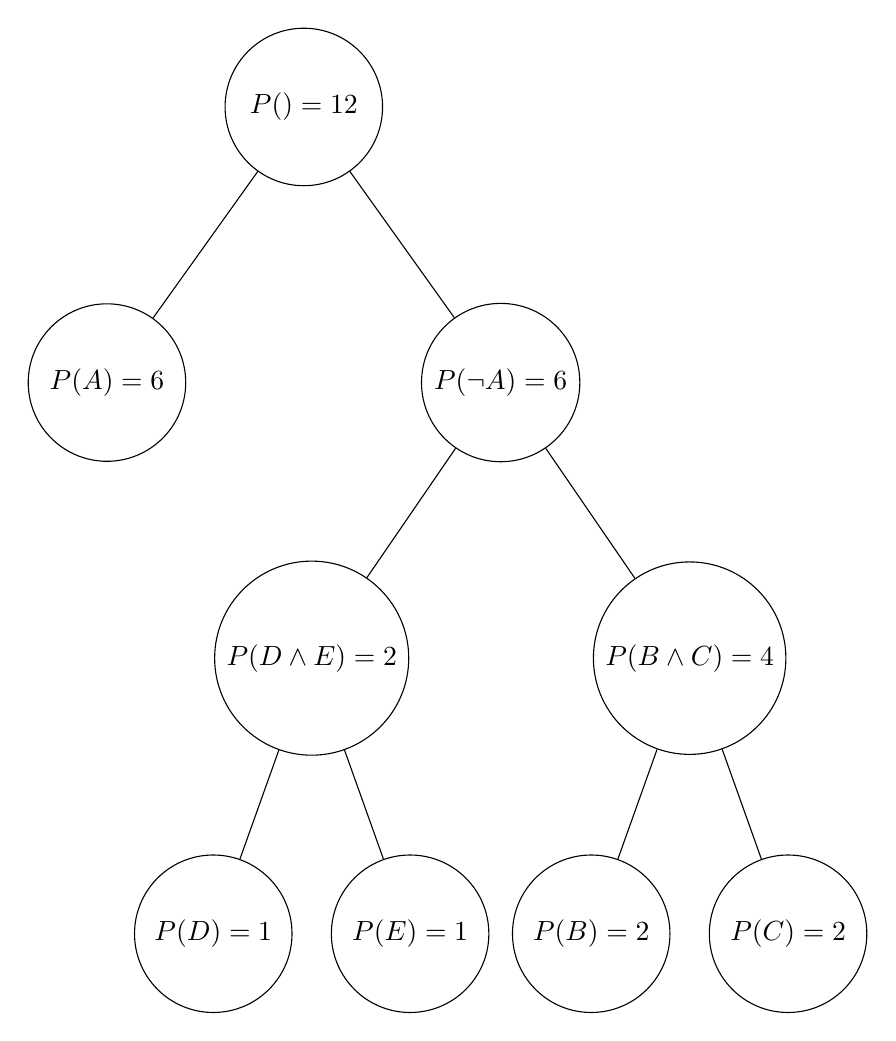
\begin{tikzpicture}[nodes={draw, circle}, 
  minimum size=2cm,
  sibling distance=3cm,
  level distance=3.5cm,
  level 1/.style={sibling distance=5cm},
  level 2/.style={sibling distance=4.8cm},
  level 3/.style={sibling distance=2.5cm}]
\node[circle,draw](z){$ P() = 12$}
  child{
	node[circle,draw]{$ P(A) = 6$}  
  }
  child{
  node[circle,draw]{$ P(\neg A) = 6 $} 
  child{
   node[circle,draw] {$ P( D \wedge E) = 2 $}
   child{
	   node[circle,draw]{$ P(D) = 1 $} 
	}
	child{
   	   node[circle,draw]{$ P(E) = 1 $} 
   }   
  }
  child{
   node[circle,draw] {$ P( B \wedge C) = 4 $}
   child{
	   node[circle,draw]{$ P(B) = 2 $} 
   }
   child{
	   node[circle,draw]{$ P(C) = 2 $}    
   } 
  } 
  };
\end{tikzpicture}

\newpage

Graph für GRIFFBRETT

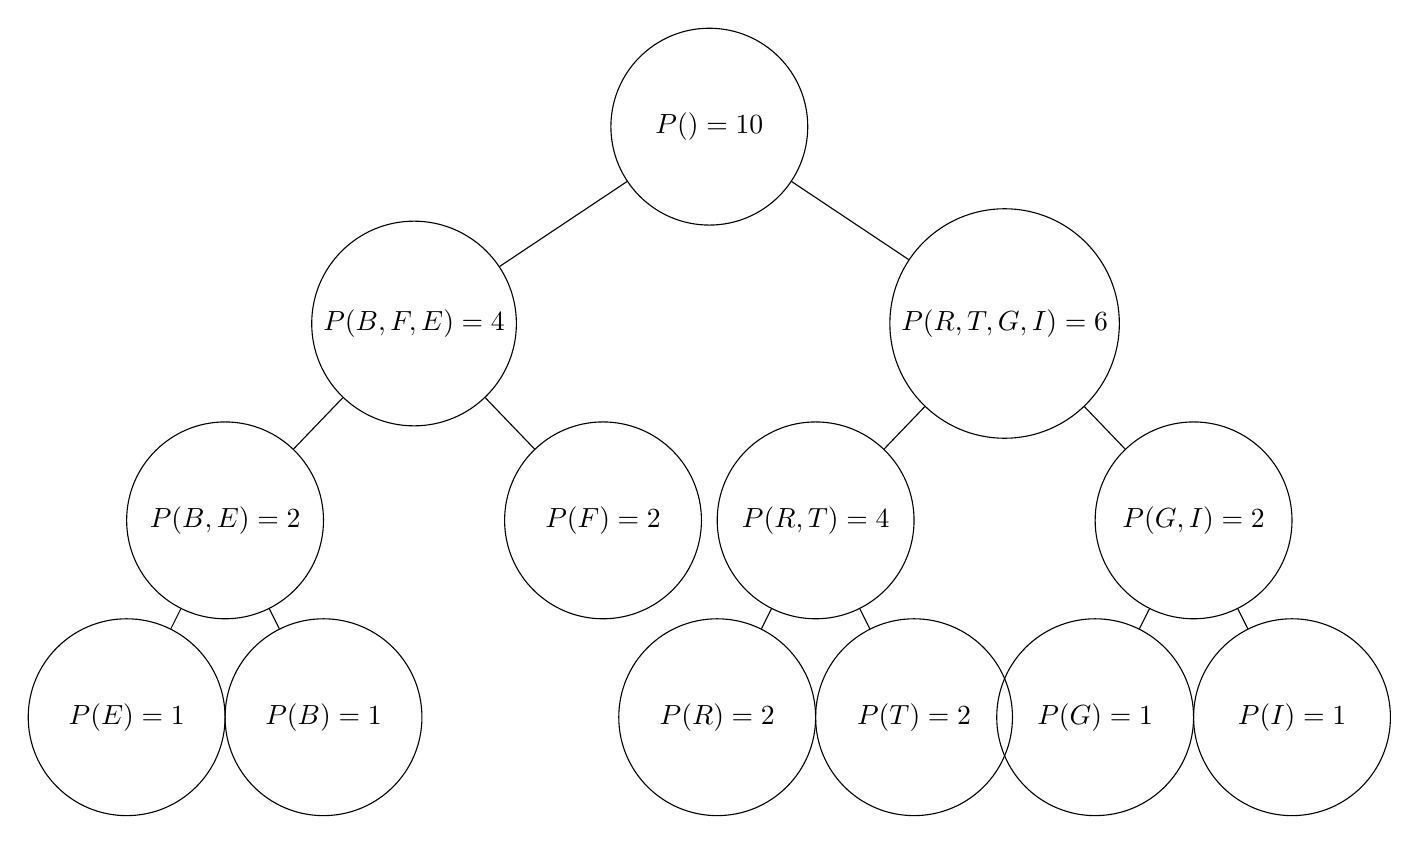
\begin{tikzpicture}[nodes={draw, circle}, 
  minimum size=2.5cm,
  sibling distance=3.5cm,
  level distance=3.7cm,level distance=2.5cm,
  level 1/.style={sibling distance=7.5cm},
  level 2/.style={sibling distance=4.8cm},
  level 3/.style={sibling distance=2.5cm}]
\node[circle,draw](z){$ P() = 10$}
  child{
	node[circle,draw]{$ P(B,F,E) = 4$}
	child{
		node[circle,draw]{$ P(B,E) = 2$}
		child{
	   		node[circle,draw]{$ P(E) = 1 $} 
		}
		child{
   	   		node[circle,draw]{$ P(B) = 1 $} 
   		}
	}	
	child{
		node[circle,draw]{$ P(F) = 2$}
	}
  }
  child{
  node[circle,draw]{$ P(R,T,G,I) = 6 $} 
  child{
   node[circle,draw] {$ P( R,T) = 4 $}
   child{
	   node[circle,draw]{$ P(R) = 2 $} 
	}
	child{
   	   node[circle,draw]{$ P(T) = 2 $} 
   }   
  }
  child{
   node[circle,draw] {$ P( G,I) = 2 $}
   child{
	   node[circle,draw]{$ P(G) = 1 $} 
   }
   child{
	   node[circle,draw]{$ P(I) = 1 $}    
   } 
  } 
  };
\end{tikzpicture}


\subsection*{Aufgabe 2b}

Das Komprimierte Wort ist: kino programm

Wir nehmen die Bitfolge gehen den Baum durch, wenn die Entscheidung welchen Ast man weiter geht, ist entschieden durch das aktuelle Bit. Den Baum gehen wir solange durch bis wir einen Blatt (Knoten ohne Kinder) finden. Das Zeichen was durch den Ast repräsentiert wird, ist das dekomprimierte Zeichen. Mit dem nächsten Bit fängt man dann wieder oben an Wurzel an und dekomprimiert das nächste Zeichen.


\end{document}